\documentclass[12pt,a4paper,titlepage,headinclude,bibtotoc]{scrartcl}

%---- Allgemeine Layout Einstellungen ------------------------------------------

% Für Kopf und Fußzeilen, siehe auch KOMA-Skript Doku
\usepackage[komastyle]{scrpage2}
\pagestyle{plain}
\setheadsepline{0.5pt}[\color{black}]
\automark[section]{chapter}


%Einstellungen für Figuren- und Tabellenbeschriftungen
\setkomafont{captionlabel}{\sffamily\bfseries}
\setcapindent{0em}


%---- Weitere Pakete -----------------------------------------------------------
% Die Pakete sind alle in der TeX Live Distribution enthalten. Wichtige Adressen
% www.ctan.org, www.dante.de

% Sprachunterstützung
\usepackage[ngerman]{babel}

% Benutzung von Umlauten direkt im Text
% entweder "latin1" oder "utf8"
\usepackage[utf8]{inputenc}

% Pakete mit Mathesymbolen und zur Beseitigung von Schwächen der Mathe-Umgebung
\usepackage{latexsym,exscale,stmaryrd,amssymb,amsmath}


\usepackage[nointegrals]{wasysym}
\usepackage{eurosym}

% Anderes Literaturverzeichnisformat
%\usepackage[square,sort&compress]{natbib}
\usepackage{hyperref}
% Für Farbe
\usepackage{color}
\usepackage{graphicx}
\usepackage{wrapfig}
\usepackage{subfigure}

% Caption neben Abbildung
\usepackage{sidecap}


% Befehl für "Entspricht"-Zeichen
\newcommand{\corresponds}{\ensuremath{\mathrel{\widehat{=}}}}
% Befehl für Errorfunction
\newcommand{\erf}[1]{\text{ erf}\ensuremath{\left( #1 \right)}}


%Fußnoten zwingend auf diese Seite setzen
\interfootnotelinepenalty=1000

%Für chemische Formeln (von www.dante.de)
%% Anpassung an LaTeX(2e) von Bernd Raichle
\makeatletter
\DeclareRobustCommand{\chemical}[1]{%
  {\(\m@th
   \edef\resetfontdimens{\noexpand\)%
       \fontdimen16\textfont2=\the\fontdimen16\textfont2
       \fontdimen17\textfont2=\the\fontdimen17\textfont2\relax}%
   \fontdimen16\textfont2=2.7pt \fontdimen17\textfont2=2.7pt
   \mathrm{#1}%
   \resetfontdimens}}
\makeatother
\usepackage{textcomp}
\usepackage{upgreek}
%\begin{document}
%$\upmu$
%\end{document}
%Honecker-Kasten mit $$\shadowbox{$xxxx$}$$
\usepackage{fancybox}

%SI-Package
\usepackage{siunitx}

%keine Einrückung, wenn Latex doppelte Leerzeile
\parindent0pt

%Bibliography \bibliography{literatur} und \cite{gerthsen}
%\usepackage{cite}
\usepackage{babelbib}
\selectbiblanguage{ngerman}

\usepackage{siunitx}
%\begin{document}
 % \SI{1.55}{\micro\metre}
\sisetup{math-micro=\text{µ},text-micro=µ}
\begin{document}

\begin{titlepage}
\centering
%\textsc{\Large Praktikum zur Einführung in die physikalische Chemie,\\[1.5ex] Universität Göttingen}

\vspace*{3cm}

\rule{\textwidth}{1pt}\\[0.5cm]
{\huge \bfseries
  V4: Molmassenbestimmung\\[1.5ex]
  durch Gefrierpunktserniedrigung}\\[0.5cm]
\rule{\textwidth}{1pt}

\vspace*{3cm}


\begin{Large}
\begin{tabular}{ll}
Durchführende: &  Alea Tokita, Julia Stachowiak\\
Assistentin: & Annemarie Kehl\\
 Versuchsdatum: & 07.12.2015\\
\end{tabular}
\end{Large}

\vspace*{2.5cm}

\begin{Large}
\fbox{
  \begin{minipage}[t][2cm][t]{6cm} 
   Werte:\\
  
  \end{minipage}
}
\end{Large}

\end{titlepage}

\tableofcontents

\newpage

\section{Theoretische Grundlagen}

Bei idealen Lösungen stehen alle Moleküle in gleicher Wechselwirkung zueinander, egal ob sie vom Lösungsmittel oder der gelösten Komponente stammen. 
Wird nun eine Größe definiert, so können verschiedene Größen der Lösung mathematisch einfach getrennt werden. Ein Beispiel hierfür ist der Dampfdruck, welcher den isothermen Druck beschreibt, unterhalb dessen eine Flüssigkeit beginnt, in den gasförmigen Zustand überzugehen.
Der Dampfdruck\,$p$ einer Komponente $i$ in der Lösung setzt sich somit aus dem Dampfdruck der Komponente\,$p_{0i}$ und dem Stoffmengenanteil\,$x_i^l$ ebendieser in der Lösung bzw. flüssigen Phase\,$l$ zusammen.
Daraus ergibt sich das Raoult'sche Gesetz:\\

\begin{equation}
p_i = P_{0i} \cdot x_i^{l}
\end{equation}
\\

Da die Moleküle in realen Lösungen immer in Wechselwirkungen zueinander treten, ist die Abweichung vom Raoult'schen Gesetz sehr groß. Eine Näherung ergibt sich nur bei sehr geringen Wechselwirkungen und daher einer sehr geringen Molalität bzw. Konzentration des gelösten Stoffes: $x_i^2\,<<1$ und daraus für das Lösungsmittel $x_1^l\,= 1 - x_2^l$. Hier wird also davon ausgegangen, dass sich die Gasphase und flüssige Phase größtenteils aus dem Lösungsmittel zusammensetzen und der Dampfdruck der gelösten Substanz somit vernachlässigbar klein ist. Somit ergibt sich aus: \\

\begin{equation}
p_{ges} = p_1 + p_2 = p_{01} \cdot x_1^l + p_{02} \cdot x_2^l
\end{equation}

näherungsweise:
\begin{equation}
p_{ges} = p_{01} \cdot (1-x_2^l)
\end{equation}

Außderdem wird davon ausgegangen, dass sich beim Lösen des Stoffes keine Unregelmäßigkeiten wie z.B. Kristalle bilden, die den Idealitätscharakter der Lösung beeinflussen würden.\\

Dampf-, Schmelz-, und Sublimationsdruck der Lösung hängen somit nicht von der Art des gelösten Stoffes, sondern nur von der Temperatur ab. So ergibt sich folgende Isochore (Abbildung 1):\\

\newpage

\begin{figure} [h!]
\begin{center}
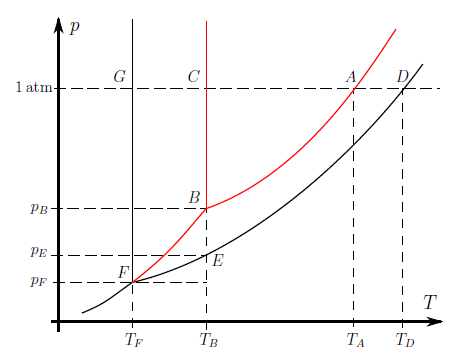
\includegraphics[scale=1]{Phasendiagramm.png} \end{center}
\caption {Zustandsdiagramm \protect\footnotemark}
\end{figure}
\footnotetext{Skriptum für das Praktikum zur Einführung in die Physikalische Chemie, Institut für physikalische Chemie, Uni Göttingen, 2015, Seite 24}

Die rote Linie zeichnet die Übergänge der Aggregatzustände des reinen Lösungsmittels. Nahe der Abszisse (dh. bei geringer Temperatur) ist der feste Bereich und nahe der Ordinate (bei geringem Druck) der gasförmige.
Somit bildet die Strecke $\overline{AB}$\,mit dem Übergang zwischen gasförmigen und flüssigem Zustand den Dampfdruck; $\overline{BC}$\,den Schmelzdruck. $\overline{FB}$\,beschreibt den Sublimationsdruck und $C$\, den Gefrierpunkt (bei\,$p= 1\mathrm{atm}$.\\
Die schwarze Kurve zeigt die Phasenübergänge der Lösung, die Bezeichnungen für die jeweiligen Streckenabschnitte gelten hier analog.\\
Auffällig ist die Verschiebung des Tripelpunktes, die nah mit der Differenz der Gefrierpunkte, dh. der Gefrierpunktserniedrigung\,$\Delta T_g = T_C - T_G$ zusammenhängt. \\
Der fast senkrechte Anstieg der Gefrierpunktserniedrigung\,$T_g$ entspricht somit näherungsweise der Verschiebung des Tripelpunktes und es ergibt sich:  \\

\begin{equation}
T_G \approx T_B - T_F
\end{equation}

Diese kann mithilfe der Steigung der Dampfdruck- und Sublimationsdruckkurven errechnet werden. Das Raoultsche Gesetz besagt:\\

\begin{equation}
p_B - p_E = p_B \cdot x_2^l
\end{equation}
\\

Für die Steigung der Dampfdruckkurve und Sublimationsdruckkurve wird ebenfalls ein linearer Verlauf angenommen. Wie auf Abbildung 1 ersichtlich besitzen sie näherungsweise dieselbe Steigung, sodass gilt:\\

\begin{equation}
\dfrac{p_B - p_E}{\Delta T_g} = \frac{\Delta p}{\Delta T}\bigg \vert_{Subl} - \frac{\Delta p}{\Delta T}\bigg \vert_{Dampf}
\end{equation}

Einsetzen der Druckdifferenz $p_B - p_E$ aus dem Raoultschen Gesetz ergibt nach Umformung für\,$T_g$:\\

\begin{equation}
\Delta T_g =\dfrac{p_B \cdot x_2^l}{\frac{\Delta p}{\Delta T}\bigg \vert_{Subl} - \frac{\Delta p}{\Delta T}\bigg \vert_{Dampf}}
\end{equation}
\\

Der Stoffmengenanteil $x_2^l$ ist proportional zur Molalität $\check c$ . Der Rest der Gleichung ist stoffabhängig und kann mit der stoffspezifischen kryoskopischen Konstante $\Theta_g$ zusammengefasst werden, welche die Schmelz- bzw. Gefierpunktsänderung darstellt:

\begin{equation}
\Delta T_g = \Theta_g \cdot \check c
\end{equation}























\end{document}


